\documentclass[10pt]{beamer}
\setbeamertemplate{navigation symbols}{\insertlogo}

%\documentclass[handout,dvips,11pt,grey]{beamer}

%\usetheme{Goettingen}
%\usetheme{Warsaw}
\usetheme{Hannover}

%\usepackage{tikz,pgf}
\usepackage{xcolor}
\usepackage{multicol}
\usepackage{amsmath,amsthm,amssymb}
%\usepackage{epstopdf}
\usepackage{xspace}
\usepackage{wrapfig}

\usepackage{verbatim}
%\usepackage{circuitikz}
%\usepackage{graphicx}
\usepackage{comment}
%\usepackage{array}
\usepackage{coffee4}


\title{Understanding and Using Topic Modeling}
\subtitle{Using inferred document clusters}
\author{Philip Robinson}
\date{September 7, 2018}
\institute{Presented to itds \\ NASA - Jet Propulsion Lab}

\DeclareMathOperator*{\argsort}{argsort}

  \logo{
\includegraphics[height=.7cm]{./logo.png}}

\begin{document}

\begin{frame}
  \titlepage

\end{frame}


\begin{frame}{Presentation Overview}
  \tableofcontents

\end{frame}

\begin{comment}
\section{Introduction}
\begin{frame}{Intern - Philip (1762)}
  Computer Science MSc at Oregon Health and Science University.

  \vspace{1em}

  \begin{multicols}{2}
    
\includegraphics[width=\columnwidth]{./philip.jpg}

    Thats me!
  \end{multicols}

\end{frame}
\end{comment}
\section{What is Topic Modeling}

\begin{frame}{What is Topic Modeling}
  {\bf Our goal: mathematically model topics from a corpus}

  \begin{quote}
    Topic modeling is a text processing technique for automatically grouping documents by topics. This is usually used as a strategy to describe documents in low dimensional space or an exploratory tool for document collections.
  \end{quote}
\end{frame}

\newcommand{\Food}[1]{\colorbox{orange!30}{#1}\xspace}
\newcommand{\Travel}[1]{\colorbox{blue!30}{#1}\xspace}
\newcommand{\Time}[1]{\colorbox{green!30}{#1}\xspace}
\newcommand{\Document}[1]{\fbox{\begin{minipage}{\columnwidth}#1\end{minipage}}}



\begin{frame}{Examples}
{\bf In practice, this requires many more documents}

  \begin{multicols}{2}

    \Document{
      The \Travel{Tourist} huddles in the \\ \Travel{station} While slowly \Time{night} gives way to \Time{dawn}; He finds a certain fascination In knowing all the \Travel{trains} are gone.
    }

    \vspace{.25em}

    \Document{
      The Governess up in the attic \\Attempts to make a cup of \Food{tea}; Her mind grows \Time{daily} more erratic From cold and \Food{hunger} and ennui.
    }

    \vspace{.25em}

    \Document{
      The Journalist surveys the slaughter, The best in \Time{years} without a doubt; He pours himself a \Food{gin} and \Food{water} and wonders how it came about.
    }

    \columnbreak

    \begin{itemize}
    \item \Food{Food}
    \item \Travel{Travel}
    \item \Time{Time}
    \end{itemize}

    \vspace{1em}

    From this annotation we know that Document 2 and 3 are about \Food{Food} and \Time{Time}
  \end{multicols}

\end{frame}

\section{Why Topic Model}
\begin{frame}{What can I solve?}
  \begin{itemize}
  \item Find similar document pairs
  \item Cluster documents into groups with similar content
  \item Find relevant documents to a query or user's interests
  \item Explore shape of document collection
  \end{itemize}

  \begin{quote}
    Topic modeling can usually be extended to address many other problems, and document embeddings can be used to inform downstream models.
  \end{quote}
\end{frame}

\begin{frame}{Applications of Topic Modeling}

  \begin{multicols}{4}

  \begin{figure}
  \includegraphics[width=\columnwidth]{full2.png}
  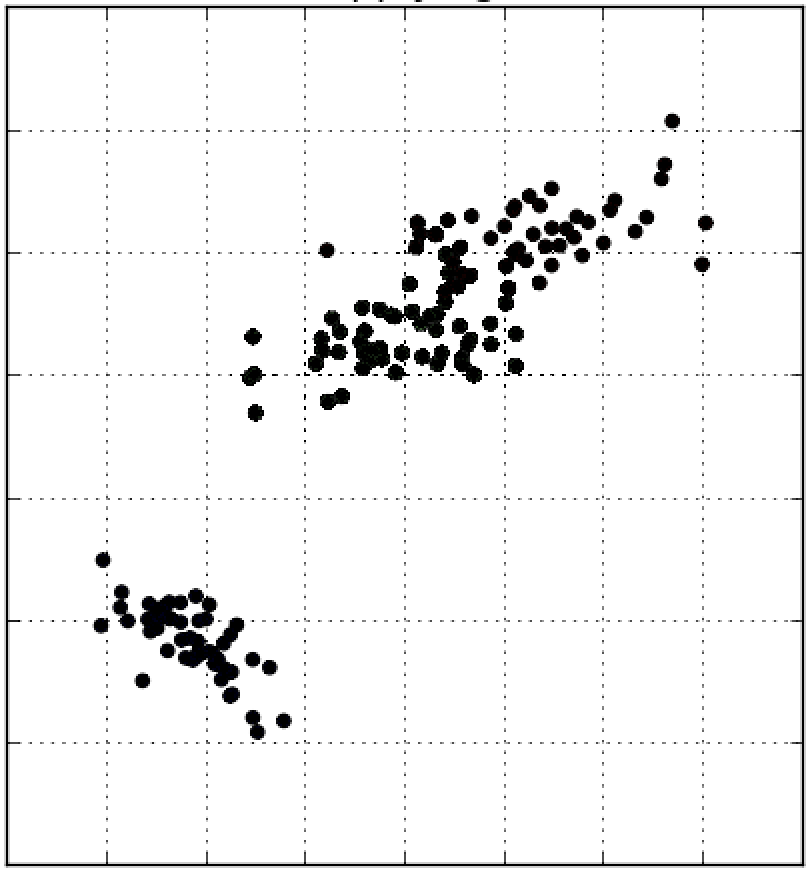
\includegraphics[width=.8\columnwidth]{reduced.png}
  \caption{Dimmentionality Reduction}
  \end{figure}

  \columnbreak

  \hfill
    \begin{figure}
  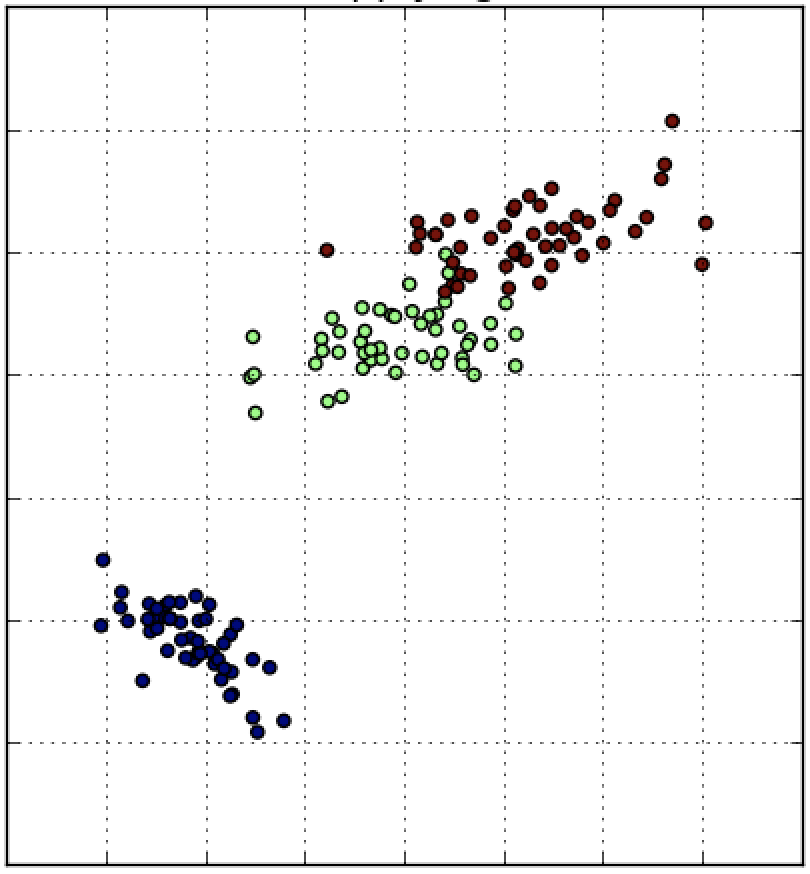
\includegraphics[width=\columnwidth]{cluster.png}
  \caption{Cluster Points}
  \end{figure}

    \columnbreak

  \hfill
    \begin{figure}
  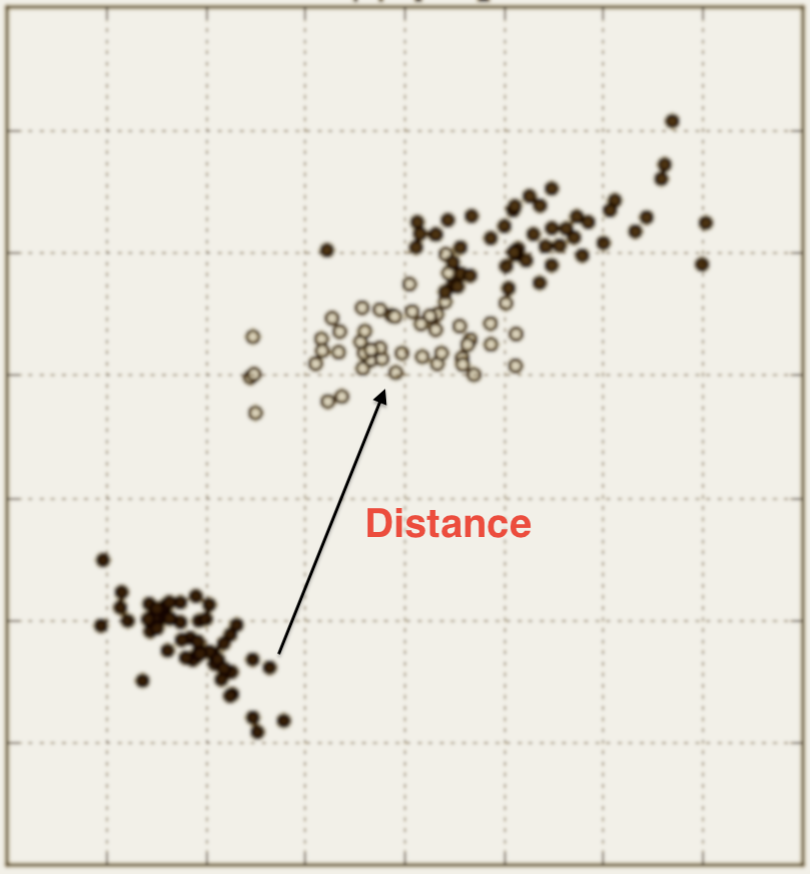
\includegraphics[width=\columnwidth]{dist.png}
  \caption{Exploratory Data Analysis}
  \end{figure}
    \columnbreak

  \hfill
    \begin{figure}
  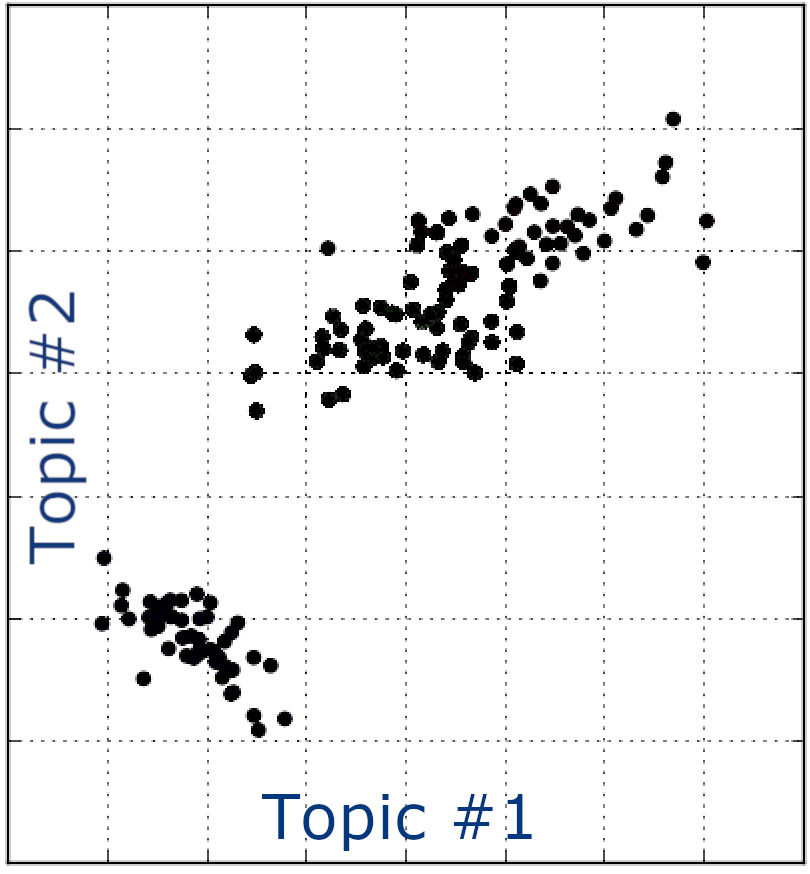
\includegraphics[width=\columnwidth]{topicanalysis.png}
  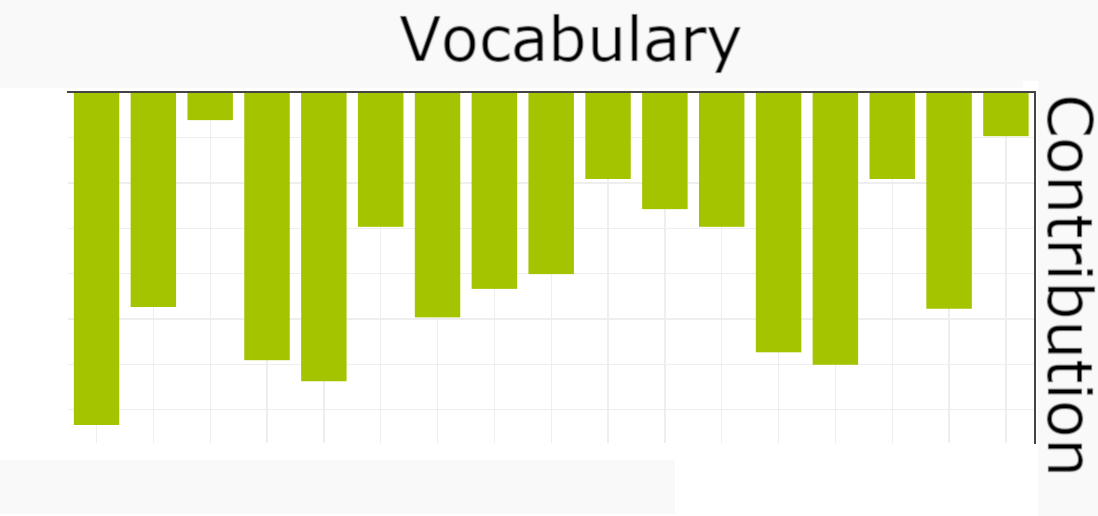
\includegraphics[width=\columnwidth]{bar-simple.png}
  \caption{Analysis of Topics}
  \end{figure}

  \end{multicols}

\end{frame}

\section{History of Topic Models}

\begin{frame}{Latent Semantic Analysis}
  {\bf SVD on Vocabulary x Document matrix}

  \begin{itemize}
  \item[{\bf Given:}] $D$ documents covering $W$ words
  \item Create $A_{DxW}$ counting or \texttt{tfidf}\footnote{
    {$a_{i,j} = tf_{i,j} \times log \frac{D}{df_j}$}
  } matrix
  \item Compute Singular Value Decomposition
  \item Select the number of description topics $t$
  \end{itemize}

  \begin{multicols}{2}
    \[A' \approx U_t S_t V_t^T\]
    \columnbreak

    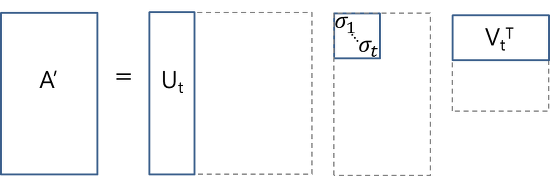
\includegraphics[width=\columnwidth]{svd.png}
  \end{multicols}
\end{frame}

\begin{frame}{Understand Latent Semantic Analysis}
  {\bf Topics are principle components of entire document collection}

  \begin{multicols}{2}
    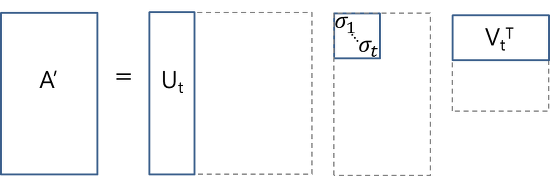
\includegraphics[width=\columnwidth]{svd.png}
    \columnbreak

    \begin{itemize}
      \item[{\bf U:}] document-topic matrix, topic contributes to document
      \item[{\bf S:}] singular values
      \item[{\bf V:}] word-topic matrix, topic contribute to words
    \end{itemize}
  \end{multicols}

  \begin{itemize}
  \item Overfit as consequence of topics strict mathematical definition
  \item Topics are better interpreted as mathematical than intuitive
  \item Cost of finding one topic is the same as finding all possible topics
  \end{itemize}


\end{frame}

\section{Generative Models}
\begin{frame}{Goals of generative models}
  {\bf A generative model}

  \begin{itemize}
  \item Assume/Generalize how data could have been generated
  \item Fit distributions that describe generalization
  \item Ask questions about the generalization in relation to data
  \item Ask questions about data in relation to the generalization
  \end{itemize}

  \vspace{1em}

  \begin{quote}
    Generative models are much easier to extend, because they abstract the model from it's linear algebra dependencies.

    \vspace{1em}

  Topic modeling generalizes how a document is generated by claiming that words come from topics, and documents have multiple topics.\footnote{this is not a language model} %Note that this ignores sentence structure, entities, authorship, or other things we may care about.

  \end{quote}

\end{frame}


\begin{frame}{Probabilistic Latent Semantic Analysis}
  {\bf Generative model for SVD}

  \[P(d,w):\rightarrow \texttt{document-term matrix}\]

    \begin{itemize}
    \item  $P(z|d)$ is the probability $z$ contributes to $d$
    \item  $P(w|z)$ is the probability $w$ contributes to $z$
    \end{itemize}

    \[P(D,W) = P(D)\sum_Z P(Z|D)P(W|Z)\]

    \[P(Z|D) \texttt{ and } P(W|Z) \sim \texttt{Multinomial}\]

\end{frame}

\begin{frame}{Understand Probabilistic Latent Semantic Analysis}
  {\bf A mapping to SVD}

  \begin{align*}
    P(D,W) &= P(D)\sum_Z P(Z|D)P(W|Z)\\
    &= \sum_Z \color{red}P(Z)\color{blue}P(D|Z)\color{green}P(W|Z)\\
    \texttt{remembering}&\\
    A &\approx\color{blue}U_t\color{red}S_t\color{green}V_t^T
  \end{align*}

  First generate the topic $Z$ then generate the word $W$

  \begin{itemize}
  \item P(D) is not parameterized, we don't observe new documents
  \item Tends to be softer than LSA, but still  overfits (grows with D)
  \item No longer use \texttt{tfidf} best replaced with \texttt{stopwords}\footnote{Usually top $.5-2\%$ of vocab}
  \end{itemize}

\end{frame}

\begin{frame}{Latend Dirichlet Allocation}
  {\bf Bayesian extension to PLSA}

  \begin{multicols}{2}

  \begin{itemize}
  \item Represent document as Bag-of-Words\footnote{equivalent to multinomial over the vocabulary}
  \item Model/Fit topics as mixture of words
  \item Documents are projected into or sampled from topic-space-distribution
  \end{itemize}

  \begin{figure}
  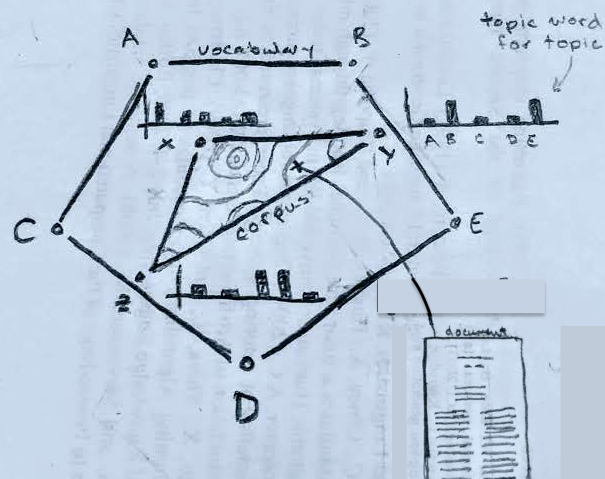
\includegraphics[width=\columnwidth]{./lda-draw.png}
  \caption{Latent Dirichlet Allocation}
  \end{figure}

  \end{multicols}

  \begin{quote}
    Enormous body of work extending this model to address more specific problems.
  \end{quote}

\end{frame}

\section{Understanding Model Space}

\begin{frame}{Dirichlet Distribution}
  {\bf In this case the Topic-Space is our Dirichlet Distribution}

    \begin{multicols}{3}

  \begin{figure}
  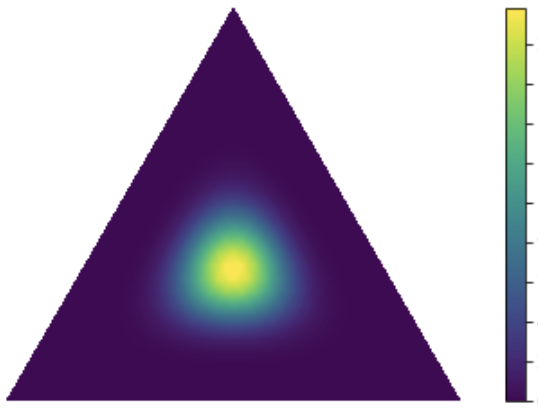
\includegraphics[width=\columnwidth]{uninformative}
  \caption{Non-Informative}
  \end{figure}

  \columnbreak

  \hfill
    \begin{figure}
  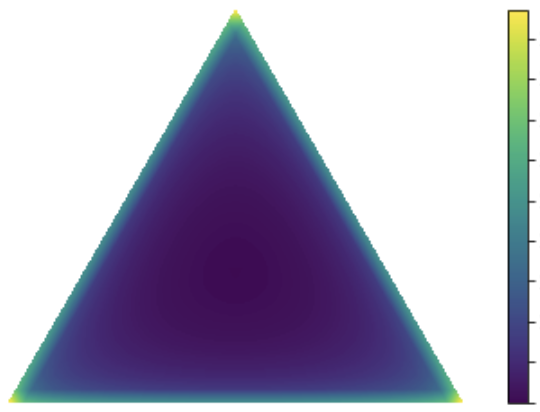
\includegraphics[width=\columnwidth]{unique.png}
  \caption{Little In Common}
  \end{figure}

    \columnbreak

  \hfill
    \begin{figure}
  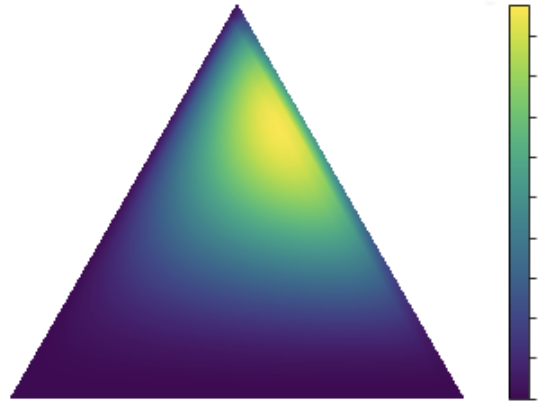
\includegraphics[width=\columnwidth]{shared.png}
  \caption{Shared Topics}
  \end{figure}

  \end{multicols}

\end{frame}

\begin{frame}{Using this in Python\footnote{example in \texttt{scikit-learn}, I used \texttt{gensim}}}
  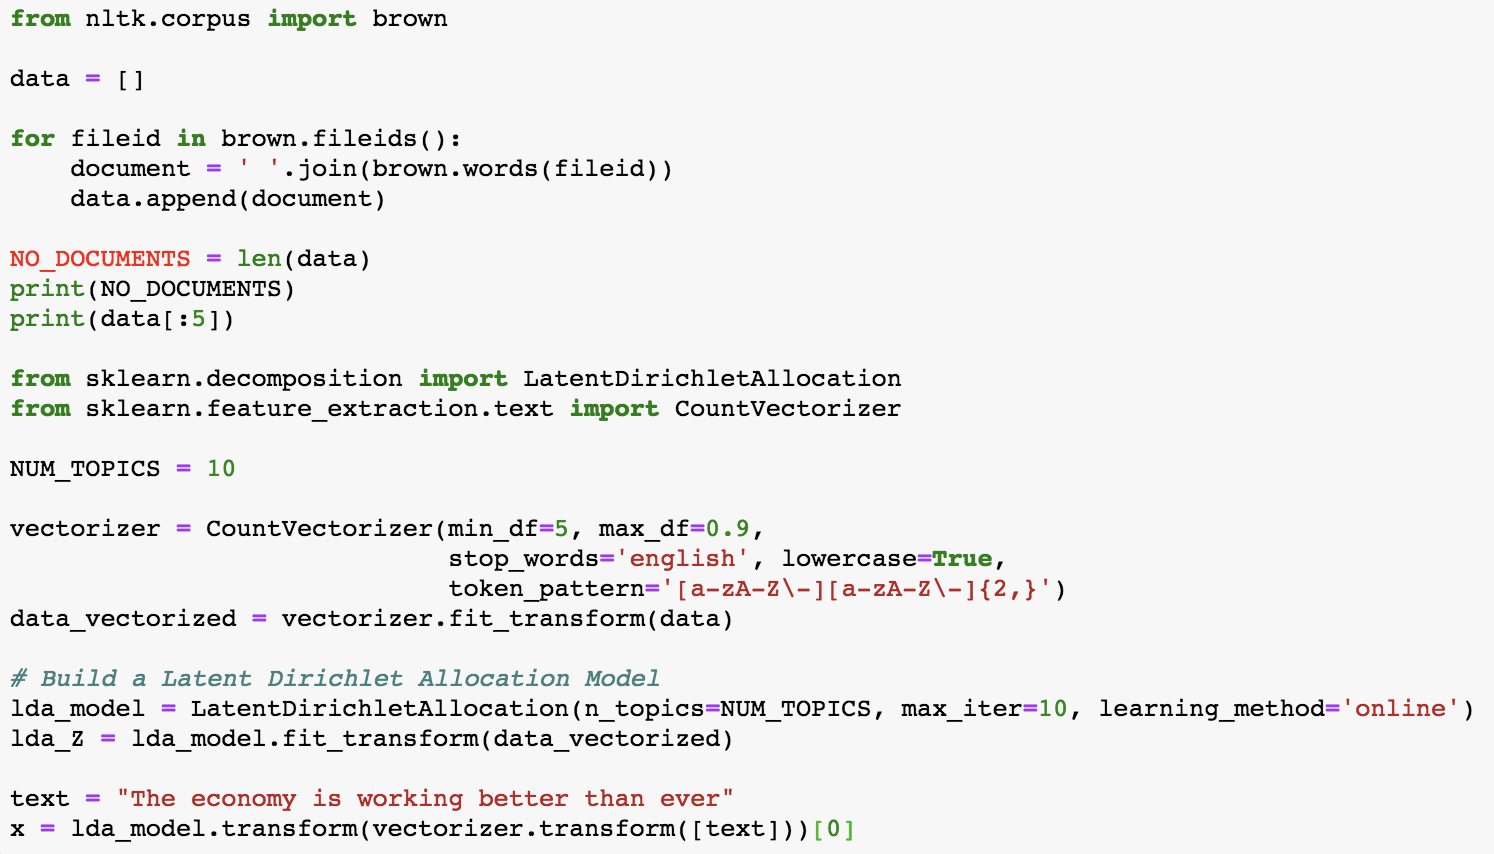
\includegraphics[width=\textwidth]{./implement.png}
\end{frame}


\begin{frame}{Looking at top words}
  {\bf Mitigating apophenia is hard, topics difficult to interpret}

  \begin{multicols}{3}
    Topic \#1
    \begin{itemize}
    \item server
    \item connected
    \item access
    \item workstation
    \item outage
    \item user
    %\item service
    %\item restart
    \end{itemize}

    \columnbreak

    Topic \#2
    \begin{itemize}
    \item mode
    \item instrument
    \item safe
    \item spacecraft
    \item anomaly
    \item recovery
    %\item event
    %\item control
    \end{itemize}

    \columnbreak

    Topic \#3
    \begin{itemize}
    \item uplink
    \item station
    \item dsn
    \item spacecraft
    \item lock
    \item ace
    %\item bps
    %\item radiation
    \end{itemize}

  \end{multicols}

  \begin{quote}
    Although the model better describes our generation process, from the perspective of topics, it can be difficult to know what these topics actually represent.\footnote{Supervised LDA attempts to addresses this\\ concern, also applies to sentiment analysis} This may require experts who are immune to apophenia.
  \end{quote}
\end{frame}


\begin{frame}{Evaluation}
  {\bf Does our fit dirichlet distribution describe our data or our understanding}

  \begin{itemize}
  \item perplexity
  \item coherence
  \item visualization
  \item predictive power
  \end{itemize}
\end{frame}

\begin{frame}{Perplexity vs Coherence}
  {\bf perplexity for prediction, coherence for EDA\footnote{exploratory data analysis}}

  \begin{quote}
    Perplexity measures how poorly the model describes the data.
  \end{quote}

  \begin{align*}
    Perplexity(q) &= b^{-\frac{1}{N}\sum_{x \in X} log_b q(x)}
  \end{align*}

  \begin{quote}
    Topic coherence measures take the set of $N$ top words from a topic and sums a \texttt{confirmation measure}\footnote{like pointwize mutual information (PMI)} over the word pairs. Probabilities are estimated from sliding window over train and test corpora.
  \end{quote}

  \begin{align*}
    C_{Irvine} &= \frac{2}{N\cdot N-1}\sum_{i=1}^{N-1}\sum_{j=i+1}^N PMI(w_i, w_j)\\
    PMI(w_i, w_j) &= log(\frac{P(w_i, w_j)}{P(w_i)\cdot P(w_j)})
  \end{align*}
\end{frame}

\begin{frame}{Interactive Visualization\footnote{used \texttt{pyLDAvis}}}
  {\bf Breakout to jupyter}

    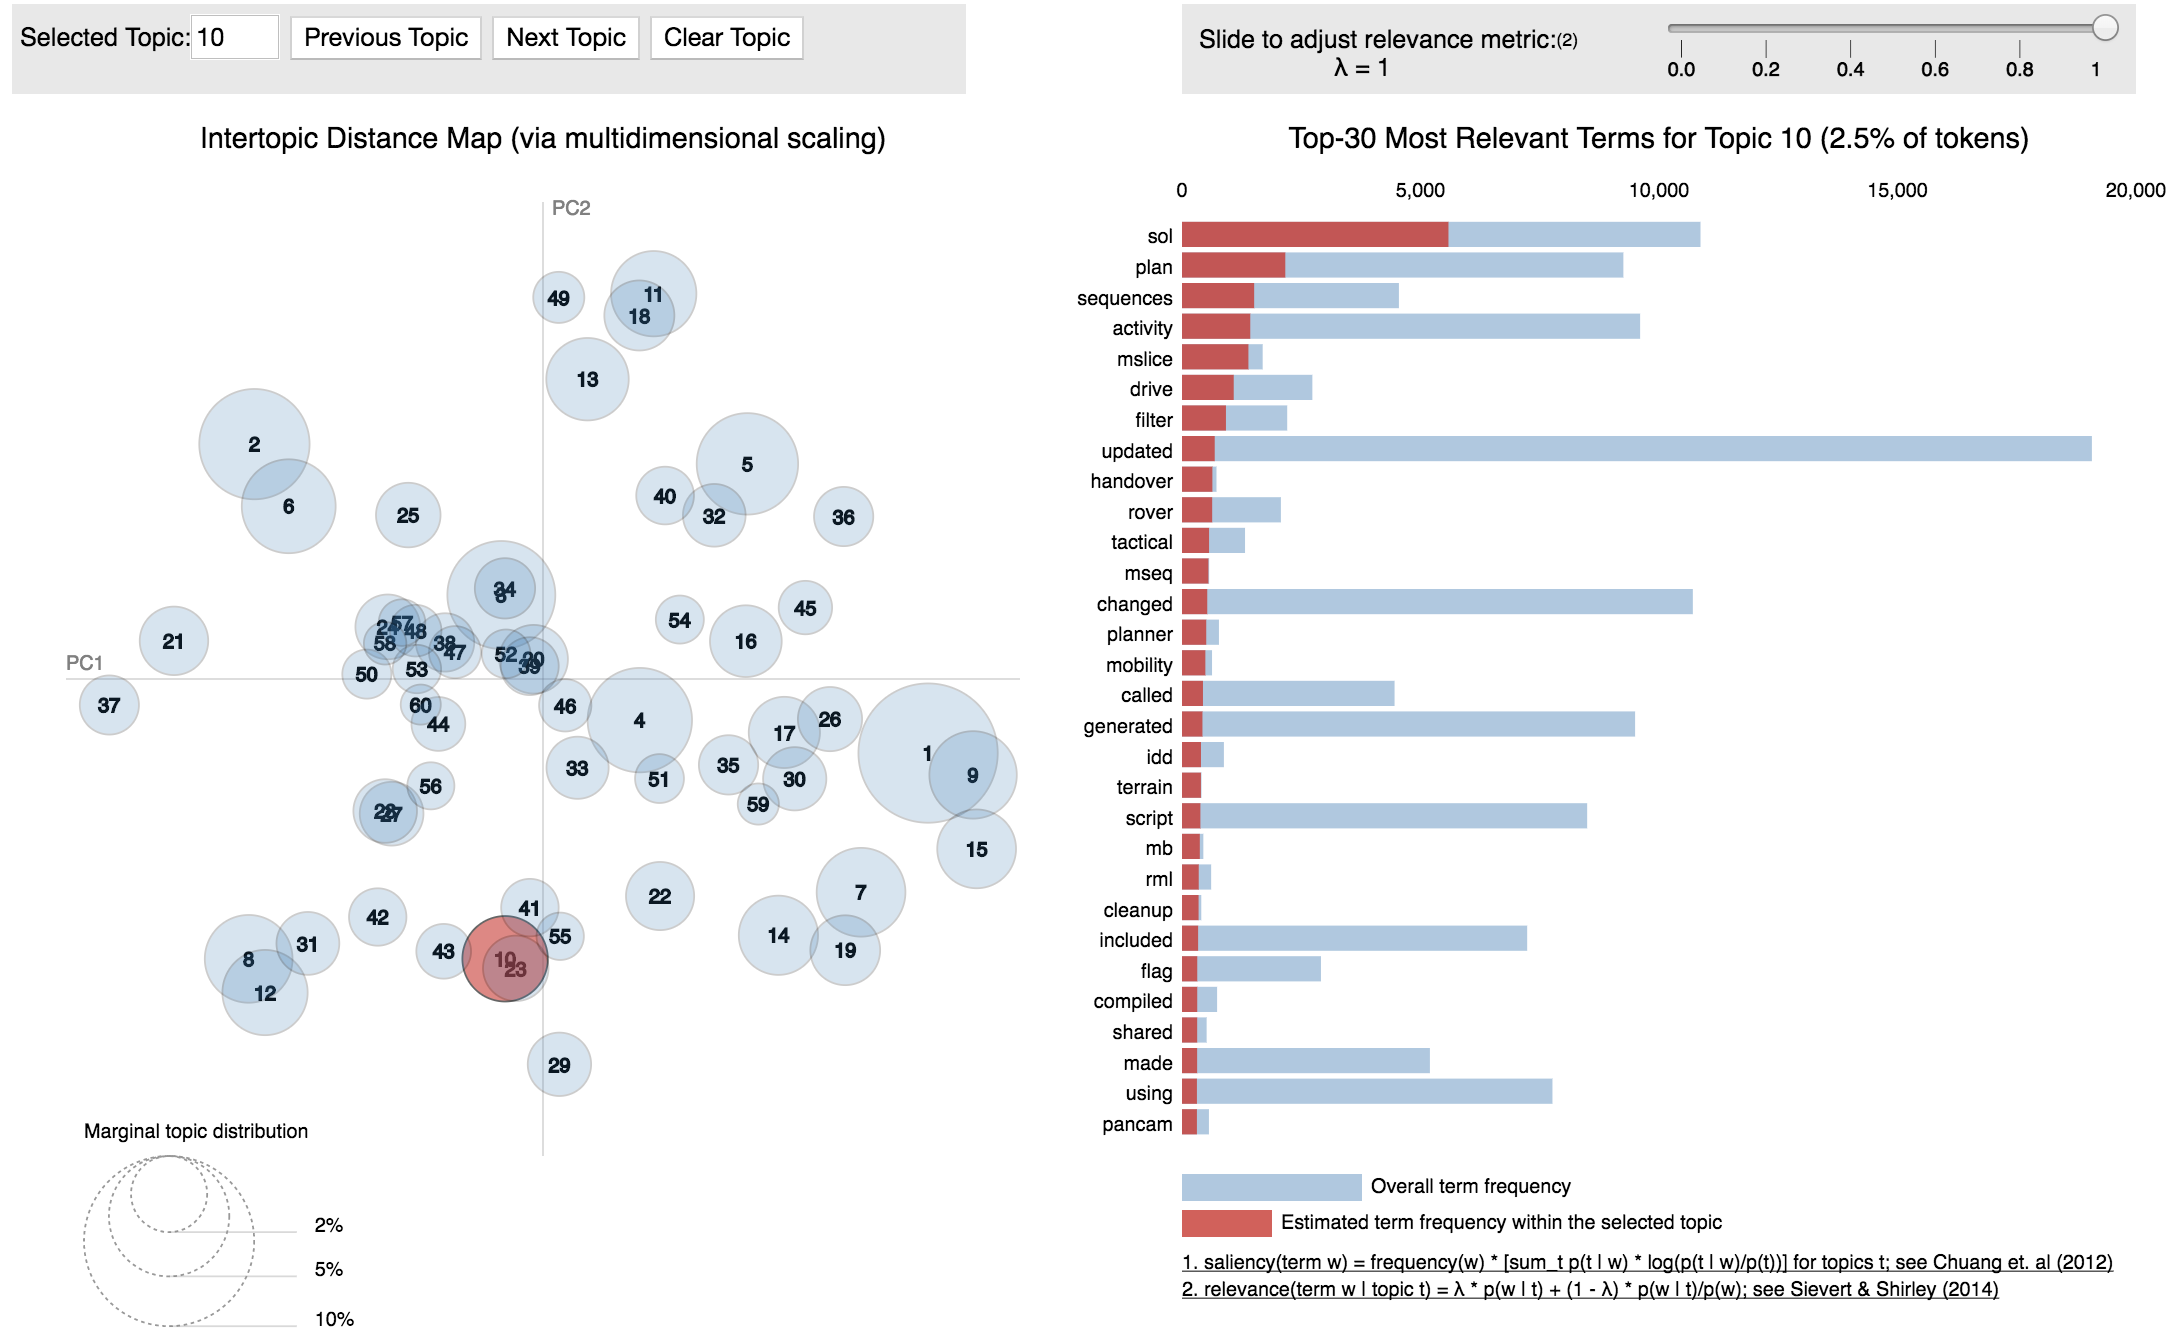
\includegraphics[width=\textwidth]{LDAvis.png}

\end{frame}

\begin{frame}{Predictive Power}
  {\bf Depends on your downstream applications}

  \begin{quote}
    Does your client end up benefiting from the tool. This could be many measures like recall or clickthrough.
  \end{quote}
\end{frame}

\section{After LDA}
\begin{frame}{Extensions}
  \begin{itemize}
  \item Correlated Topic Model
  \item[$\rightarrow$] Author Topic Model
  \item Biterm Topic Model
  \item Hierarchical Dirichlet Process
  \end{itemize}
\end{frame}

\section{Pitfalls}

\begin{frame}{Distance Measures}
  {\bf Testing distances is cheaper than understanding them}

  \begin{quote}
    Hellinger distance is a distance between probability distributions. The domain of the Dirichlet distribution can be thought of as a simplex over multinomial distributions.\footnote{Most online examples use cosine distance, \\without justification}
  \end{quote}
\end{frame}

\begin{frame}{Text Pre-Processing}
{\bf Cleaning applies to most 'simple' NLP problems}

\begin{quote}
  Text normalization is custom to your corpus. Many of the steps are the same, but their application changes with the type of documents.
\end{quote}

  \begin{itemize}
  \item Normalize text
    \begin{itemize}
    \item Lowercase text
    \item[$\star$] Remove non-informative text patterns
    \end{itemize}
  \item Tokenization \& (Stemming | Lemmatization)
    \begin{itemize}
    \item[$\star$] pick a stemmer
    \item Stem \hfill\texttt{(applies, applying, apply) -> (appli)}
    \item[$\star$] Un-Stem \hfill\texttt{(appli) -> (apply)}
    \end{itemize}
  \item Focus corpus (remove ``stop words``)
    \begin{itemize}
    \item drop most frequent words
    \item \texttt{nltk} english stop-words
    \item Remove extremely rare words
    \end{itemize}
  \end{itemize}

\end{frame}

\begin{frame}{Non-Informative Delinquent Cases}
  {\bf Evaluation metrics are only informative given reasonable parameters}

  \begin{quote}
    You can often reduce perplexity by having fewer topics.
    Maximizing coherence is more resilient to this effect.
  \end{quote}
\end{frame}

\begin{frame}{Verifying your intent}
  {\bf You may not need interpretable topics!}

  \begin{quote}
    Base LDA, on it's own, isn't that great. Understanding LDA allows you to understand the extensions, which are pretty cool.
  \end{quote}

  \vspace{2em}

  \begin{quote}
    Not all evaluation metrics have been written for the extensions, so you may have to come up with proxies.
  \end{quote}

\end{frame}

\begin{frame}{Stability of Topics}
  \begin{quote}
    If you are extremely dependent on understandability, then you may need to incorporate model stability.\footnote{http://doi.acm.org/10.1145/2954002}
  \end{quote}
\end{frame}

\section{Conclusion}

\begin{frame}{Take Away}

\begin{itemize}
\item Perform text level EDA to customize cleaning processing
\item Pick a model type
\item Evaluation takes care
  \begin{itemize}
  \item Identify a model-fit measure
  \item Identify a performance strategy
  \end{itemize}
\end{itemize}

\vspace{2em}

\begin{quote}
Simply put, LDA attempts to generalize truncated SVD with a generative bias to how we write papers.
\end{quote}
\end{frame}


\begin{frame}{Conclusion \& Questions}

  \begin{quote}
    I used the Author Topic Model during my internship to automatically assign tickets to subject matter experts, for the Office of Safety and Mission Success (5x)
  \end{quote}

\end{frame}

\end{document}
